\chapter{Realizace}
\label{ch:implementation}
V rámci této kapitoly se budeme zabývat konečným výběrem technologií a architekturou aplikace. Správným výběrem technologií a kvalitním návrhem aplikace zajistíme snadnou rozšiřitelnost aplikace a zároveň zpřehledníme kód.


\section{Použité technologie}
\label{sc:used_techologies}
Pro vývoj samotné aplikace byl využit TypeScript, pro frontend framework React v~kombinaci s~Apollo Client\footnote{https://www.apollographql.com/} a pro backend Node.JS, konkrétně knihovnu Express\footnote{https://expressjs.com/} a Apollo Server\footnote{https://www.apollographql.com/} a pro komunikaci GraphQL. K~vývoji však patří ještě další podpůrné nástroje, kterými se zabývají následující sekce, stejně jako podrobnějšímu popisu již zmíněných technologií.

\subsection{GraphQL}
\label{ss:graphql}
GraphQL, kde \emph{QL} je zkratka pro Query Language, je dotazovací jazyk. Jedná se o~jazyk vyvíjený přímo pro použití v~\acrshort{api}, původně vyvíjený firmou \emph{Facebook}, dnes již pod neziskovou organizací \emph{GraphQL Foundation}. Na rozdíl od standardního \acrshort{rest} API, které umožňuje získání, nebo úpravu jednoho objektu pomocí specifické cesty, tak GraphQL server naslouchá jedné cestě a jako parametr dostává stromovou strukturu zapsanou ve speciálním formátu. Tento přístup má mnoho výhod, umožňuje vývojáři vybrat si přímo jaká data požaduje (a tím snížit datový tok), také umožňuje slučování více požadavků do jednoho, silné typování samotného \acrshort{api} endpointu což umožňuje našeptávání a statickou kontrolu. Nevýhoda oproti REST \acrshort{api} je využití jedné cesty a tím znemožnění cachování na straně prohlížeče. \cite{brito2020rest}

Ve spojitosti s~GraphQL se budeme bavit o~požadavcích typu \uv{query} a \uv{mutace}. Query je obdobou GET požadavku REST \acrshort{api}, tedy pouze získá data. Mutace na druhou stranu je obdoba POST, UPDATE nebo DELETE požadavku, tedy jakákoliv operace, která nějak manipuluje s~daty. Oba typy mohou mít proměnné a vracet nějaké hodnoty. Existuje ještě jeden specifický typ požadavku, \uv{subscription}, který umožňuje navázat trvalé spojení a dostávat okamžitá upozornění na nová data. Tento typ požadavku avšak není potřebný pro tento typ aplikace, hodí se však kdekoliv, kde je třeba upozornit na změny okamžitě, např. chat. \cite{porcello_2018_learning}

\subsection{MongoDB a Mongoose}
\label{ss:mongoose}
MongoDB\footnote{https://www.mongodb.com/} je NoSQL databáze. Hlavní výhoda NoSQL databází je rychlejší vývoj a prototypování, jelikož se nemusí žádným způsobem vytvářet tabulky. Výhodou MongoDB je přístup k~ukládání dat, a to ve formě dokumentů, kde každý dokument je tvořen z~dvojic klíče a hodnoty. Takovýto dokument je až na typy shodný s~JSON, tedy propojení MongoDB a javascriptové aplikace je triviální.

Mongoose\footnote{https://mongoosejs.com/} je tzv. \acrfull{orm} nástroj vytvořený firmou \emph{Automattic} přímo pro databázi MongoDB. To umožňuje vytvořit jednotlivé datové modely ze schémat. Schéma je objekt definující vlastnosti modelu, jako jsou pole, indexy, validace, virtuální pole a další \cite{automatticinc_2020_mongoose}. Takto vytvořený model poskytuje možnost vytvářet, vyhledávat, upravovat či mazat záznamy v~databázi.

Další a největší výhodou tohoto přístupu vytváření modelů je možnost z~takových modelů automaticky vytvořit GraphQL mutace a query a to za použití knihoven \emph{graphql-compose} a \emph{graphql-compose-mongoose}. Tyto knihovny vytvoří základní query a mutace pro vyhledávání či úpravu modelů, které jsou snadno rozšiřitelné o~další, vlastní, operace nad modely.

\subsection{Yarn v2}
\label{ss:yarn}
Yarn\footnote{https://yarnpkg.com/} je alternativa k~\acrshort{npm}, což je balíčkovací systém pro JavaScript, obdoba NuGetu pro C\# nebo Mavenu pro Javu.

Od verze 2.0, taky zvané \emph{berry}, integruje podporu tzv. monorepozitáře, tedy přístupu kdy jeden repozitář obsahuje několik podprojektů. Tuto možnost poskytuje i nástroj \href{https://github.com/lerna/lerna}{\emph{Lerna}}, kde se vývojáři~\nameref{ss:yarn} inspirovali. To vede k~možnosti modularizace aplikace a zavedení Single responsibility principu.

Další podstatná funkcionalita Yarn v2 je vynucená podpora \acrfull{pnp} režimu. \acrshort{pnp} je přístup zavedený týmem hlavních vývojářů Yarnu. Při standartní instalaci balíčků pomocí npm nebo yarn bez pnp, jsou balíčky staženy a rozbaleny do adresáře \emph{node\_modules} ze kterého potom čerpá \acrfull{nra}~\cite{joyentinc_1_noderesolutionalgorithm}. Tento algoritmus při sestavování výsledné aplikace pro každé volání funkce \emph{require()} vždy projde složku \emph{node\_modules} a pokud daný balíček nenajde, pak rekurzivně pokračuje v~nadřazeném adresáři (za předpokladu, že nadřazený adresář obsahuje složku \emph{node\_modules}). Tento přístup je i s~nějakými optimalizacemi velmi pomalý. Yarn s~\acrshort{pnp} provádí to, že při prvotní instalaci závislostí místo vytvoření \emph{node\_modules} složky, kam by se následně rozbalovaly balíčky, tak vytvoří vlastní adresář \emph{.yarn/cache} kam stáhne balíčky, nerozbaluje je a následně vytvoří soubor \emph{pnp.js} který uchovává odkazy na všechny balíčky a závislosti. Výhodou je až o~70\% vyšší rychlost a menší zatížení disku a procesoru při instalaci. Nevýhodou je, že všechny instalované balíčky musí mít explicitní výpis všech svých závislostí, což velká část do dnešní doby nemá a spoléhá na to, že jejich závislosti prostě budou k~dispozici a \acrshort{nra} je najde.

Jelikož Yarn v2 ještě nevyšel jako stabilní verze, nýbrž pouze jeho release kandidáti, tak se k~němu špatně hledají informace v~případě potíží. Další problém, který tento přístup přinesl do práce, byla nutnost opravy chybějících závislostí některých balíčků. Jak již bylo zmíněno, každý balíček musí mít seznam svých závislostí a když nemá, tak sestavení selže. Takže je na každém vývojáři, aby tyto závislosti doplnil a to formou zápisu do konfiguračního \emph{.yarnrc.yml} souboru, kde je v~práci takto opraveno zhruba 30 závislostí. Výhodou pak je mnohem rychlejší instalace závislostí, sestavení aplikace a podpora monorepozitáře.

\subsection{Express}
\label{ss:express}
Express je minimalistický webový framework pro Node.js. Jedná se o~jednoduchý webový server, který dokáže obsluhovat standardní http požadavky. Umožňuje, mimo jiné, jednotlivým cestám nastavit middleware, což jsou funkce, které jsou spuštěny před samotným vyhodnocováním funkce k~dané cestě. Typickým využitím je autentizace uživatele, nebo zapisování do log souboru. V~rámci aplikace byl použit jak pro poskytování backend, tak i frontend serveru. Backend server poskytuje GraphQL \acrshort{api} a zajišťuje napojení na databázi, zatím co frontend server poskytuje \acrfull{ssr} aplikace. Co znamená \acrshort{ssr} se budeme podrobněji zabývat v~rámci samostatné sekce~\ref{ss:ssr}.

\subsection{Apollo Server}
\label{ss:apollo_server}
Apollo Server je GraphQL server vyvíjený společností \emph{Meteor Development Group, Inc.}, který je nezávislý na volbě webového serveru, v~našem případě~\ref{ss:express}, který je takzvaně \emph{unopinionated}, což znamená, že vývojáře netlačí nějakou specifickou cestou vývoje. Jeho hlavní výhodou je hlavně jednoduchost, ale i popularita, tedy větší komunita. Menším detailem, který potěší hlavně vývojáře, je automatické vystavování GraphQL Playground, což je webová aplikace umožňující simulování dotazů, které má funkce jako IDE, tedy našeptávání, kontrola typů, kontrola syntaxe, \ldots{}.

\subsection{Apollo Client}
\label{ss:apollo_client}
Apollo Client\footnote{https://www.apollographql.com/} je od stejné společnosti jako~\ref{ss:apollo_server} a tyto dvě knihovny nejlépe fungují právě, když jsou pohromadě. Mezi hlavní výhody Apollo Client patří snadné cachování, velké množství dalších balíčků od komunity, nebo správa lokálního stavu aplikace, kterému se budeme věnovat podrobněji v~sekci~\ref{ss:local_state_management}.

\subsection{React}
\label{ss:react}
Konečná volba padla na React hlavně z~důvodu největší popularity, a tedy i největší podpory ze strany komunity. V~rámci této práce je již zakomponováno několik technologíí, které nejsou zatím se stabilním stavu a je tedy mít nějaký styčný bod, na který je možný plně spoléhat. I~z~toho důvodu byla použita stabilní verze Reactu a ne \emph{nightly} nebo \emph{experimentální}, které sice poskytují některé pěkné funkcionality, např. \emph{Concurrent Mode} zrychlující render aplikace nebo \emph{Suspense} zjednodušující čekání na asynchronní úkoly, ale výsledná aplikace by byla nestabilní, což by pro vývoj znamenalo značné zdržení.


\subsection{Storybook.js}
\label{ss:storybook}
Tato knihovna umožňuje vytvářet interaktivní dema k~jednotlivým React komponentám. Každá komponenta může obsahovat story soubor, který specifikuje, jak se má daná komponenta zobrazit a případně nastavení k~dalším pluginům. Tyto story soubory jsou následně načteny, seřazeny do stromové struktury a z~toho je následně vytvořena interaktivní dokumentace. Tato dokumentace je velmi přehledná a zároveň nutí vývojáře izolovat komponenty, což opět vede implementaci Single responsibility principu. Jednotlivé pluginy rozšiřují možnosti například pro generování dokumentace z~JSDoc komentářů nebo aby jednotlivé story byly součástí jednotkových testů.

\subsection{Jest}
\label{ss:jest}
Jest\footnote{https://jestjs.io/} je testovací knihovna pro JavaScript vyvíjená společností Facebook. Umožnuje psát jednotkové testy, simulovat data, generovat reporty pokrytí kódu ale hlavně, má ze všech testovacích knihoven pro JavaScript nejlepší podporu testování React komponent.


\section{Architektura systému}
\label{sc:system_architecture}
Jak již bylo zmíněno v~nefunkčních požadavcích, aplikace má být lehce rozšiřitelná. Tomuto požadavku se dá vyhovět několika způsoby, avšak ideologii JavaScriptu se nejvíce blíží je modularizace \cite{bevacqua_2018_mastering}. A~pro lepší přehlednost kódu a zjednodušení testování samotných modulů, se jednotlivé moduly řídí metodikou~\nameref{ss:clean_architecture}.

\subsection{Modularizace}
Aplikace byla modularizována tak, že nejprve byla rozdělena na jednotlivé domény, které je možné vidět na obrázku~\ref{fig:class_diagram}. Následně tyto domény byly rozděleny na tři části, backend, frontend a společné.

\begin{figure}
    \centering
    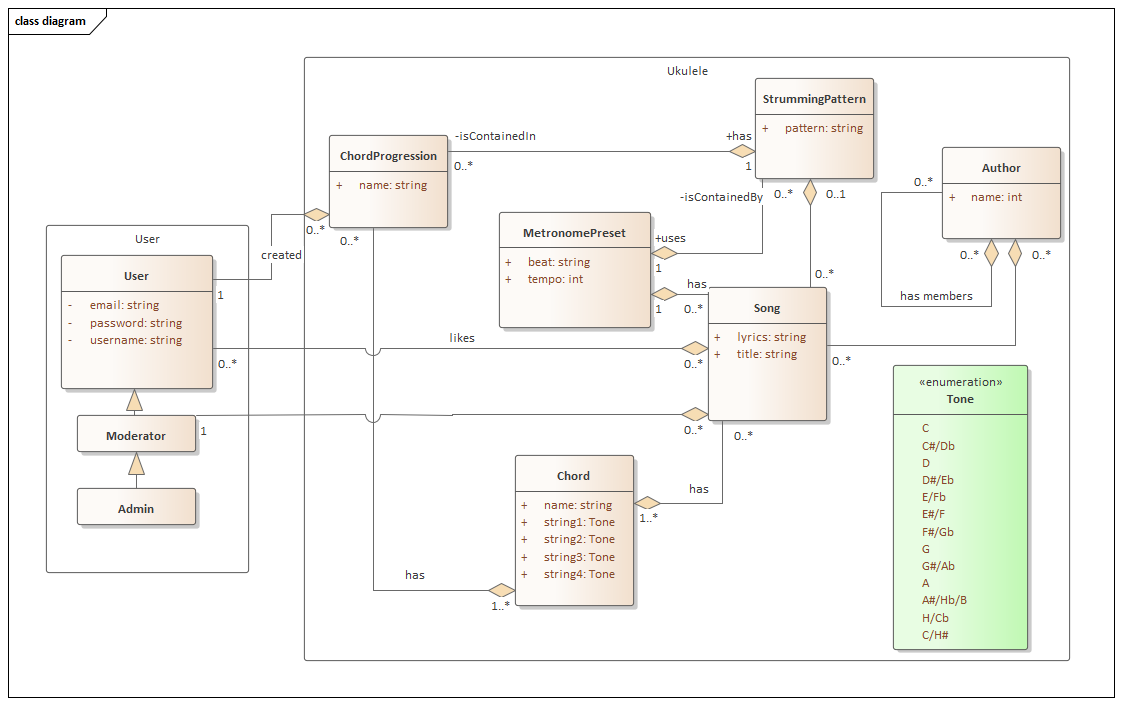
\includegraphics[width=\textwidth]{assets/class_diagram.png}
    \caption{Diagram tříd znázorňující domény}
    \label{fig:class_diagram}
\end{figure}

Backend část specifikuje veškerou práci s~daty, která se odehrává na serveru, od validace až po vystavování mutací a query pro GraphQL server. Tato část smí být závislá jen na společné části domény a modulu autorizace. Díky tomu se zajistí striktní oddělení domén a zjednoduší testování, jelikož jednotkové testy pak testují jen skutečně jednu funkcionalitu nezávisle na všech ostatních. Každý takovýto balíček exportuje jednu funkci, která jako parametr dostane nastavení a vrací objekt obsahující \emph{seed} pro inicializaci aplikace, mutace a query pro GraphQL server.

V~části frontend jsou vytvořeny jednotlivé komponenty, zase pouze pro jednu danou doménu. Tato část je závislá pouze na společné části domény, na modulu autorizace a na modulu \emph{look}, který udává vzhled aplikaci, tím že obsahuje základní komponenty, jako například tlačítko nebo základní vstupní pole. Takovýto balíček exportuje dané komponenty.

Takto rozdělené části tvoří balíčky. Tyto balíčky na sobě závisí, tak jak bylo popsáno výše a tyto závislosti jsou spravovány právě pomocí~\ref{ss:yarn} jako monorepo. Jednotlivé balíčky mají unifikované jména, a to takto:~\sloppy{\emph{uls@<doména>-<react|nodejs|common>}} kde uls je zkratka pro \emph{ukulele learning site}, což je pracovní název aplikace.

Jednotlivé balíčky ovšem netvoří výslednou aplikaci, proto je potřeba mít ještě další dva speciální balíčky, jeden pro backend a druhý pro frontend. Backend balíček importuje všechny inicializační funkce, vytvoří inicializační parametry, vytvoří jednotlivé moduly a následně je registruje do GraphQL serveru. Frontend balíček nejen, že importuje všechny komponenty, ale následně je skládá na stránky. Jednotlivé komponenty tedy neví, v~jakém kontextu a kde budou zobrazeny, a proto je potřeba aby byly správně zapouzdřené a komunikovali jen pomocí vstupních parametrů. Top level balíček, který je nadřazený všem, vytváří pouze testovací prostředí a slouží jako root balíček pro všechny moduly tak, aby mohlo správně fungovat monorepo.


\begin{figure}
    \dirtree{%
        .1 root projektu.
        .2 modules\DTcomment{Adresář s~moduly}.
        .3 look\DTcomment{Modul udávající vzhled aplikace}.
        .4 react.
        .3 ukulele\DTcomment{Modul obsahující doménu hry na ukulele}.
        .4 common.
        .4 nodejs.
        .4 react.
        .3 \ldots .
        .2 packages.
        .3 nodejs\DTcomment{Sestavuje backend server}.
        .3 react\DTcomment{Sestavuje frontend server}.
    }
    \caption{Zjednodušená adresářová struktura}
    \label{fig:modules}
\end{figure}

\subsection{Clean Architecture}
\label{ss:clean_architecture}
Tato metodika, prezentovaná ve stejnojmenné knize od R. C. Martina~\cite{martin_2018_clean}, popisuje jak rozdělit aplikaci na jednotlivé vrstvy. Říká, že aplikace by měla být rozdělena na \emph{entity}, \emph{use case}, \emph{presenters, controllers} a \emph{frameworks, drivers}, znázorňující obrázek~\ref{fig:clean_architecture}.
Entity definují základní byznys pravidla dané domény a jejich reprezentace může být například sada funkcí, nebo objekt s~metodami nebo bez. V~rámci této práce jsou entity reprezentovány pomocí objektů bez metod, přesněji TypeScript interfaces, a to hlavně z~důvodu snadné serializace a deserializace.
Vrstva use case provadí operace specifické pro aplikaci nad danými entitami. V~případě této práce to jsou \emph{intereactory}, třídy které manipulují s~entitami.
Následující vrstva už převádí dané entity na objekty vhodné pro další vrstvu frameworků, jedná se tedy o~interface. V~této práci je tato vrstva Mongoose modely, se kterými následně pracuje databáze a zároveň ze kterých se generuje GraphQL API, kterým backend předává informace frontendu. A~poslední vrstvou jsou samotné frameworky či databáze, v~případě této práce se jedná o~React, resp. MongoDB, které informace zobrazují, resp. ukládají.

Výhodou tohoto rozdělení je přehlednost a snadné testování. Při testování dané vrstvy, se vždy přistupuje z~vrstvy nadřazené, test tedy simuluje operace, které by dělala vrstva nadřazená a mockuje se první podřazená vrstva. Je tedy vždy jasné, jak daný test funguje a jaká data testuje. V~případe těchto testů mluvíme o~testech jednotkových, nikoliv smoke nebo integračních.

\begin{figure}
    \centering
    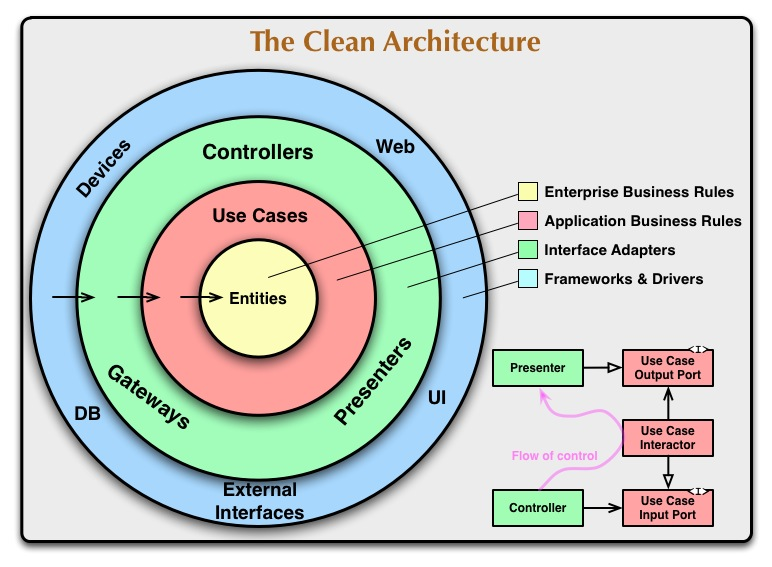
\includegraphics[width=\textwidth]{assets/clean_architecture.jpg}
    \caption{Clean Architecture \cite{martin_2019_clean}}
    \label{fig:clean_architecture}
\end{figure}



\section{Backend}
\label{sc:backend}
Realizace samotného backendu nebyla náročná a to právě díky vhodně zvoleným technologiím. Většina potřeb byla vyřízena pouhým definováním mongoose schémat, ze kterých se následně vytvořili modely a z nich GraphQL schéma. Úprav modelů bylo minimum, jako příklad takové úpravy by mohlo být smazání pole hesla z modelu uživatele při vracení daného modelu. Tato úprava je vidět na ukázce \ref{code:to_json_user}, kde je k metodě \mintinline{typescript}{toJSON}, přidaný transformátor, který vytvoří \emph{UserInteractor ui} a zavolá \mintinline{typescript}{ui.stripUser()}. Tato metoda pouze pouze vrátí kopii původního uživatele bez hesla.

\begin{figure}[h!]
    \centering
    \begin{minted}{javascript}
UserSchema.set('toJSON', {
    transform: function(doc: any, ret: any, opt: any) {
        const ui = new UserInteractor(ret);
        return ui.stripUser();
    },
});
    \end{minted}
    \caption{Odebrání hesla z modelu uživatele}
    \label{code:to_json_user}
\end{figure}

Největší problém bylo provázání modulů, tak aby na sobě byly nezávislé ale zároveň poskytovali všechny funkcionality. Konkrétně se jednalo o modul uživatele a výuky, například kvůli \ref{FP24}, který vyžaduje propojení jednotlivých modulů. Tento TODO

\section{Frontend}
\label{sc:frontend}

\subsection{Lokalní správa stavu aplikace}
\label{ss:local_state_management}

\subsection{SSR}
\label{ss:ssr}

\subsection{Themes}
\label{ss:themes}


